\chapter{Background}

\section{Video Encoding}

Computer storage and processing power is often obtained at a premium. While this is less true today, as reliable high-capacity hard disk and solid-state drives have become widely available, high definition raw video footage still places a large constraint on these high-capacity drives. They can quickly become filled with only a few minutes of content. For example, a 1080p video has a frame resolution of 1920x1080, meaning a single frame consists of 2,073,600 pixels. Each pixel is represented by three values; one for red, one for blue, and one for green. For standard 8-bit color, a single pixel requires 24 bits of storage. Thus, a single frame requires 49,766,400 bits or about 6 Megabytes of storage. Videos are often played at 24, 30, or even 60 frames per second (fps). A raw 1080p video at 24 fps requires 142.4 Megabytes of storage per second of content. A 1 Terabyte hard drive could store only 122 minutes of content, or a little over 2 hours, whereas a 1 Terabyte hard drive could hold upwards of 350 hours of video compressed by H.264. If the video was 30 or 60 fps, then the maximum capacity of the hard drive would be even less.

Thus there is a need to be able to compress video files such that they retain the same or similar visual quality while being tens or hundreds of times smaller, depending on the use case. The information stored in video files has a large amount redundancy. This redundancy is primarily along two axes, spatial and temporal. Video compression standards smartly exploit these redundancies to produce highly compressed video files. Two popular video codecs are MPEG-2 \cite{mpeg2}, used in DVDs and H.264 \cite{h264}, used for encoding high definition video.

Spatial redundancy in video is similar to that of still images. Most of the information in the visual domain in an image is encoded in low frequency components. One can reduce the amount of information in the high frequency regions of an image and incur very little perceptual loss while reducing the overall size of the image. Joint Photography Experts Group (JPEG) encoding is a widely used compression standard for images that makes use of this particular phenomenon. A simple way to encode video is to treat each video frame as a still image, and encode it using a JPEG-like process. One of the first video encoding standards, Motion JPEG, did this. However, this method of video compression does not reach the levels of compression when exploiting both spacial and temporal redundancy.

Temporal redundancy is exploiting the fact that in most cases, one video frame does not change too much from the previous frame or frames. Often portions of a video will remain completely static, while certain sections move (think a traffic camera). As such, for a sufficiently small time interval, the current frame can be predicted from the previous frame. Obviously, the current frame is not an exact match for the previous frame. Thus, the difference between the two frames, referred to as the prediction error residual, is stored alongside the previous frame. As shown in Fig.~\ref{residualvis}, an error residual for a small amount of motion has an extremely low dynamic range. Most values are black, or close to it. It is possible then, to also highly compress the residual frame using a JPEG-like process to get even more space savings without losing much in the way of prediction accuracy.

\begin{figure}[htbp]
\centerline{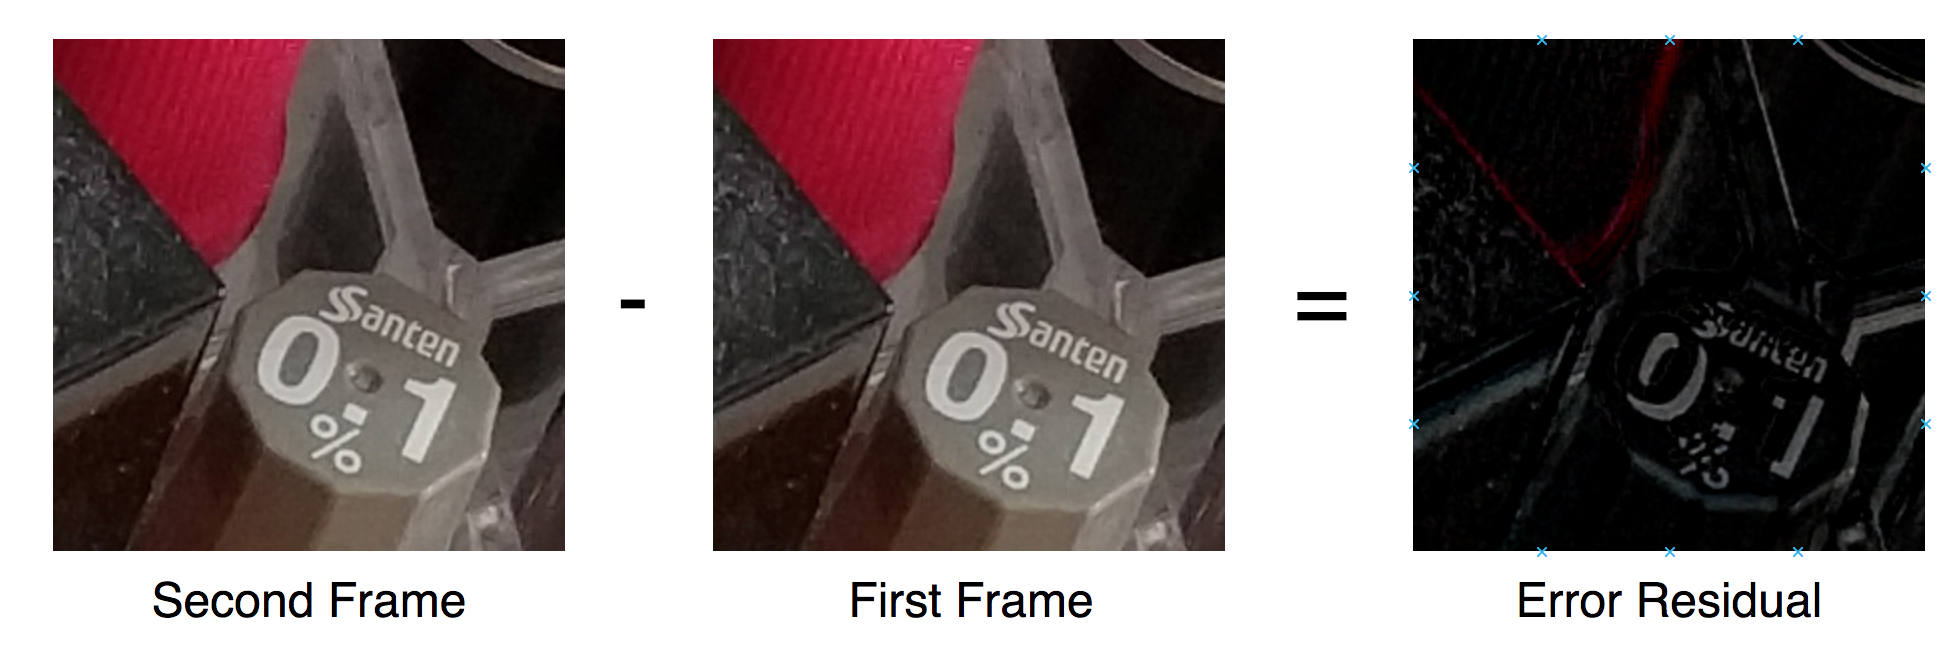
\includegraphics[width=0.9\linewidth]{Background/error_residual_vis.png}}
\caption{Visualization of a Video Prediction Error Residual}
\label{residualvis}
\end{figure}

MPEG-2 takes both of these concepts a step further. Both temporal and spatial redundancy are exploited in the frame prediction process. Successive video frames are first grouped together to minimize prediction error. The first frame in the group is encoded entirely using a JPEG-like process. This frame is called an intra-coded frame or I-frame. Following this I-frame is a sequence of predicted frames. Predicted frames come in two types. Regular predicted frames or P-frames derive their predictions from past frames. Bi-directional frames, or B-frames can mix predictions from both past and future frames. These groupings of frames are called groups of pictures (GOPs).

\begin{figure}[htbp]
\centerline{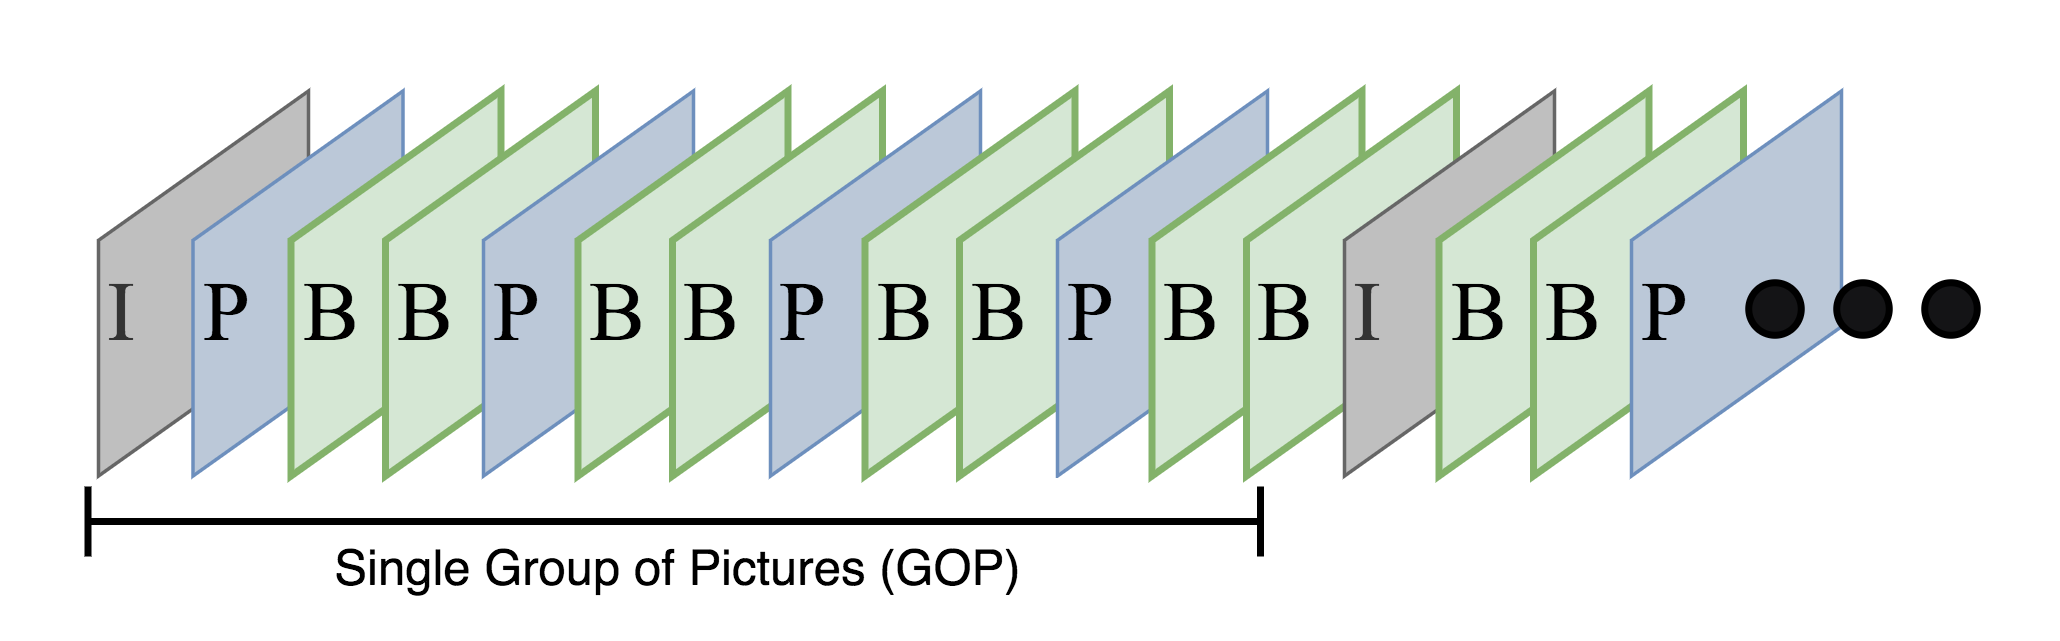
\includegraphics[width=0.9\linewidth]{Background/gop_example.png}}
\caption{Example of a GOP Sequence}
\label{exampleGOP}
\end{figure}

An example GOP sequence can be seen in Fig.~\ref{exampleGOP}. In most modern codecs, including MPEG-2, these GOP structures do not have to be fixed in size. The GOP length is determined by the distance between subsequent I-frames. Often, it is more efficient to make the GOP smaller during segments of high motion in a video. This is known as variable GOP encoding, versus fixed GOP encoding where the GOP sequence is always the same length.

Predictions can only be derived from I or P-frames, sometimes referred to as anchor frames. In MPEG-2, P-frames can only derive their predictions from a single previous anchor frame, while B-frames can derive their predictions from both a single previous and a single future anchor frame \cite{mpeg2}. To decrease the prediction error, predicted frames are partitioned into 16x16 pixel regions called macroblocks. These macroblocks are compared with blocks in the previous anchor frame and/or the next anchor frame in the case of B-frames. A fast search algorithm is performed to find a macroblock sized region with the smallest error when subtracted from the macroblock of interest.

The pixel displacement in both the x and y directions from the centroids of the macroblocks is stored in what is known as a motion vector. Then the error residual between the two macroblocks mapped by the motion vector is also stored. In this way, predicted frames are transmitted as a set of motion vectors and macroblock sized prediction error residuals. Decoding a predicted frame requires using the motion vectors to obtain the pixel values of the source macroblock for each macroblock in the frame. Then the error residual for each macroblock is added back, thus reproducing the original picture. The entire prediction error and motion vector generation process is known as motion compensation and estimation.

The H.264 specification contains many advancements in the motion compensation and estimation process \cite{h264} \cite{h264Overview}. Macroblocks no longer have to be 16x16 pixel blocks, and instead can be a variety of shapes including 8x16, 16x8, and 8x8. Single macroblocks can be encoded like an I-frame, instead of being predicted. These I-blocks are useful in scenes with high motion. Also, macroblocks can derive predictions from other portions of their frame. Intra-frame predictions are useful for large, mostly single colored regions like the sky. In this way, only one inter-frame motion vector has to be produced for an entire section of the image. It is also possible for the encoder to entirely skip a prediction for a given macroblock. Instead, the macroblock is directly copied from a previously decoded frame. These are known as skip macroblocks, or S-blocks.

The most notable improvement from H.264 over MPEG-2 is the ability for the encoder to have a substantially larger frame buffer. This allows for macroblocks in predicted frames to derive the motion vectors from across multiple different anchor frames. Effectively, a B-frame could be composed of macroblocks sourced from all anchor frames in the encoder's frame buffer. This substantially reduces the prediction error of any given macroblock. Fig.~\ref{multipred} shows an example of this. The first B-frame can source macroblocks from any I and P-frame within the GOP that is resident in the encoder's frame buffer.

\begin{figure}[htbp]
\centerline{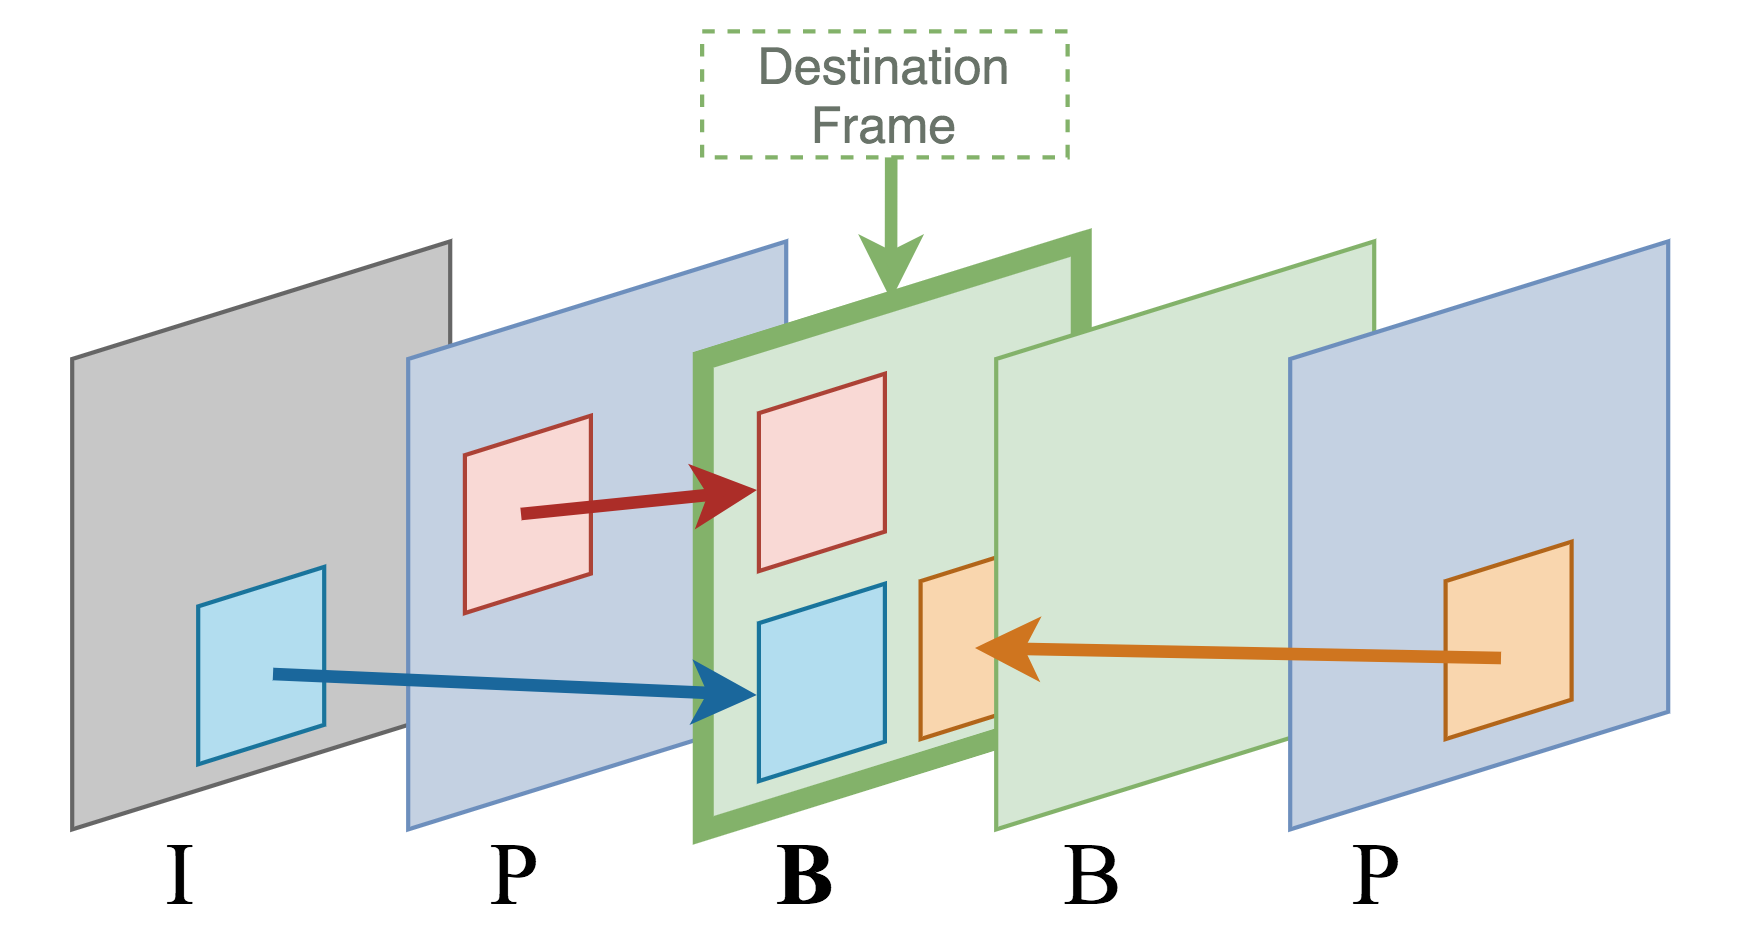
\includegraphics[width=0.9\linewidth]{Background/multi_frame_pred.png}}
\caption{Visualization of Using Multiple Anchor Frames for Prediction in H.264}
\label{multipred}
\end{figure}

\section{Frame Deletion Detection}

Detecting the tampering of a video uses similar general techniques that were originally used for detecting tampering in images. In most cases, a statistical fingerprint is extracted from the media source which contains information about the specific method of tampering an investigator wishes to detect. Frame deletion detection in video was originally found to create two distinct fingerprints in the underlying video \cite{wang}. 

One of these fingerprints is spatial in nature. When a video has had frames removed from it using video editing software, the video must first be decoded. One can simply store the decoded video without recompression, but then they would run into storage limitations as shown previously. Thus, it is common to recompress a video after removing frames. In this manner, detecting frame deletion in video is related to detecting double compression of video. Due to the JPEG-like process of encoding I-frames, Wang and Farid show that a similar fingerprint to the one used to detect double JPEG compression \cite{doubleJPEG} \cite{doubleJPEG2} is found in the I-frames of doubly compressed MPEG video. Note that this fingerprint occurs even if no frames are removed from the video \cite{wang}. Thus, more information is needed to determine whether or not a video has had frames removed from it.

The temporal fingerprint observed by Wang and Farid can make this distinction \cite{wang}. The temporal fingerprint occurs due to the structure of the motion compensation and estimation process in MPEG-2 encoding. In each GOP, the statically compressed I-frame is inserted to prevent excessive buildup of motion estimation errors. The first P-frame in a GOP is thus directly encoded with respect to the I-frame. As each subsequent P-frame in the GOP is encoded based on the previous P-frame, it can be said the these P-frames are indirectly encoded with respect to the initial I-frame. As well, the content of each P-frame is found to be correlated with the I-frame. Wang and Farid explain this phenomenon as the result of the JPEG-like compression process of the I-frame \cite{wang}. The compression artifacts propagate through the P-frames resulting in each P-frame being correlated to its previous anchor frame. In addition, the correlation between P-frames in different GOPs is reduced compared to the correlation within a single GOP.

\begin{figure}[htbp]
\centerline{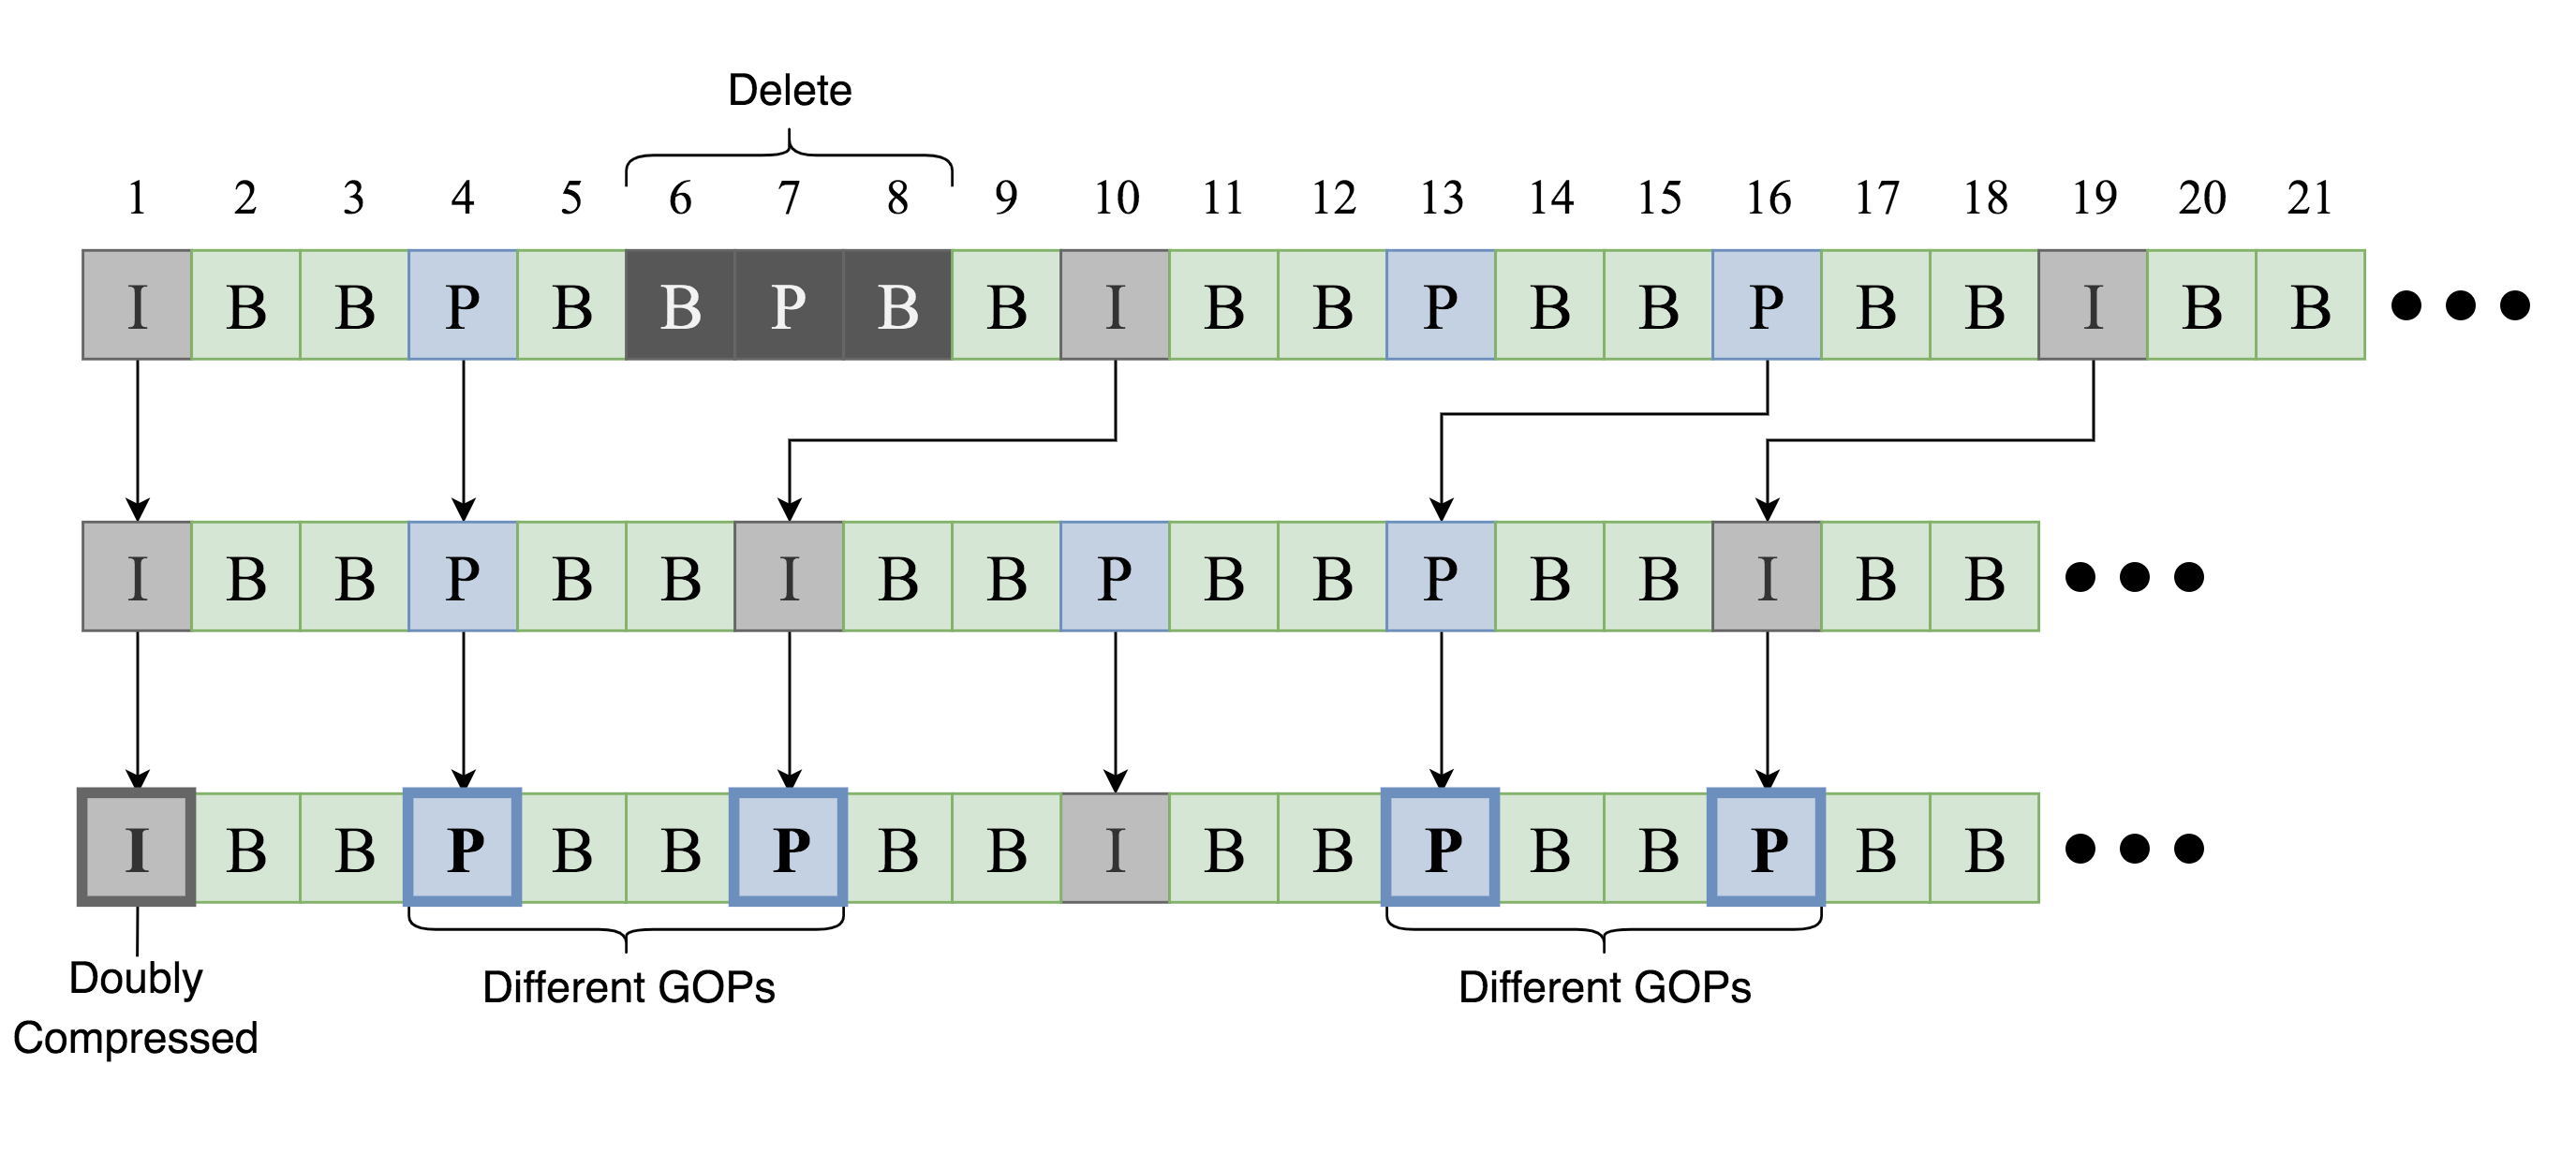
\includegraphics[width=0.9\linewidth]{Background/frame_deletion.png}}
\caption[Visualization of the Effects of Frame Deletion on a Sample MPEG-2 Encoded Video.]{Visualization of the effects of frame deletion on a sample MPEG-2 encoded video. The top row shows the original encoded sequence, while the bottom rows show the effects of deleting the three highlighted frames.}
\label{framedeletion}
\end{figure}

When frames are removed from a video, the new sequence of frames has GOPs that contain frames from across multiple GOPs in the original unaltered video. As a result, some frames can change type, and predicted frames can derive their predictions from frames originally in another GOP. This effect can be seen in Fig.~\ref{framedeletion}. Frames 6-8 were removed from the original video sequence. Note that frame 13 has become an I-frame when it was originally a P-frame, and frames 10 and 19 have become P-frames when they were originally I-frames. When frames derive their predictions across GOP boundaries, the correlation between the frames is lower, and thus there is an increase in prediction error. Wang and Farid show that for fixed GOP videos, this increase is periodic with respect to the length of a GOP.

As such, Wang and Farid proposed observing the average inter-frame prediction error for each P-frame in a given video. If there are periodic spikes in this P-frame prediction error sequence, then the video has had frames removed from it. While Wang and Farid showed that this fingerprint exists, they did not formulate a detection algorithm for this fingerprint, nor did they test the effects of frame deletion on variable GOP video. They relied on visual inspection of the Discrete Fourier Transform (DFT) of the P-frame prediction error sequence for detecting frame deletion.

Further work was done by Stamm et al. \cite{stamm} \cite{C} on using the temporal fingerprint proposed by Wang and Farid to detect frame deletion in MPEG-2 video. Stamm et al. proposed an initial model for the fingerprint itself, and how to separate an estimate of the fingerprint from a given P-frame prediction error sequence. They then formulated two decision rules based on the estimated fingerprint signal. One was for fixed GOP video, and the other was for variable GOP video. The variable GOP decision rule was found to also work for fixed GOP video as well, since it was based on the total energy in the estimated fingerprint signal.

This work still had limitations. First, it is not clear whether this detection method is robust to advancements in video encoding, particularly the ability for H.264 to derive motion vectors across multiple anchor frames. As well, both Stamm et al. and Wang and Farid were limited in the type of data they were able to generate for their experiments. They both used video with carefully controlled processing histories that are not necessarily representative of video that can be found in real world scenarios.

\subsection{Frame Deletion Detection on H.264}

Work on frame deletion detection in more modern video codecs, such as H.264 or MPEG-4 so far has been limited. Techniques have been proposed based on Wang and Farid and Stamm et al.'s original solutions for MPEG-2. However, they only cover video without B-Frames and the scenario where the altered video undergoes recompression with a different GOP size after frames have been removed \cite{Liu}. Another technique based on detecting mismatches in image sensor based traces within a video \cite{Mandelli} is able to detect video splicing, where content is stitched together from multiple camera sources. However, this technique may not work on video take only from one camera, as well as video that has undergone motion stabilization, a post-processing technique found in many smartphone cameras.

Of particular note is a technique proposed V\'azquez-Pad\'in et al. \cite{Vazquez} They found that when H.264 video is reencoded, particularly when GOP sizes do not match between encodings, the number of I-blocks and S-blocks vary from expected values when P-frames are encoded as I-frames and vice-versa. V\'azquez-Pad\'in et al. showed that it is possible to use this mismatch to determine whether an H.264 video has been recompressed \cite{Vazquez}. This technique was expanded upon by Gironi et al. \cite{barni}. As videos that have undergone frame deletion will naturally have frames change type upon reencoding, the same mismatch in the number of expected I and S-blocks appears in videos with frame deletion as well. Gironi et al. reformulated the proposed fingerprint by V\'azquez-Pad\'in et al. to work in this context. However, the method proposed by Gironi et al. is unable to work on video that has a variable GOP size.

\section{Autoregressive Models}

In our proposed frame deletion detection technique we use a statistical forecasting model called an autoregressive (AR) model. Here we describe how it works. An AR model is a statistical model of a stochastic process. The model seeks to predict future values of the process based on past observations. They are used for forecasting when there is some correlation between the values within the process. The future values are modeled as a linear combination of past observations (called lag variables) and white noise. You only use data from the same process to model the future values, thus the name "autoregressive". Effectively an AR model is a linear regression of the past data in a stochastic process where the target value is a future value of the process.

The model order of an AR model depends on the number of lag variables used in calculating the future values. Thus for a $M^{th}$ order AR model, the current value of the time series $u(n)$ is defined as

\begin{equation}
u(n) = \sum_{k = 1}^{M} w^{*}_{k} u(n-k) + v
\end{equation}

where $w^{*}_{1}, \dots, w^{*}_{M}$ are the AR model parameters $v$ is white noise. The variance of the white noise component determines the degree to which the model is able to fit the stochastic process. AR models are solved using the Yule-Walker equations as found in \cite{ARmodels}. In this work, we use the AR model parameters for a given video to characterize the properties of the frame deletion fingerprint. In doing so, we are able to account for the natural variance between videos in our decision-making process.

\section{Support Vector Machines}

In order to make a decision as to whether a video has had frames removed from it, we use a Support Vector Machine (SVM) classifier. SVMs are a widely popular machine learning technique for classification \cite{svm}. The goal of an SVM is to learn an optimal separating hyperplane between classes of data by maximizing the margin between the data points in each class that are closest to data points in the other classes. These closest points are known as support vectors. The support vector machine learns a discriminate function based on these support vectors. The SVM does not make a probabilistic model of the data to determine classification. However, there are techniques \cite{plattscaling} to scale the data in such a fashion that the SVM can return an estimate of the probability that a data point is from a particular class. Fig.~\ref{svmvis} shows an example of creating a binary decision function  using an SVM.

\begin{figure}[htbp]
\centerline{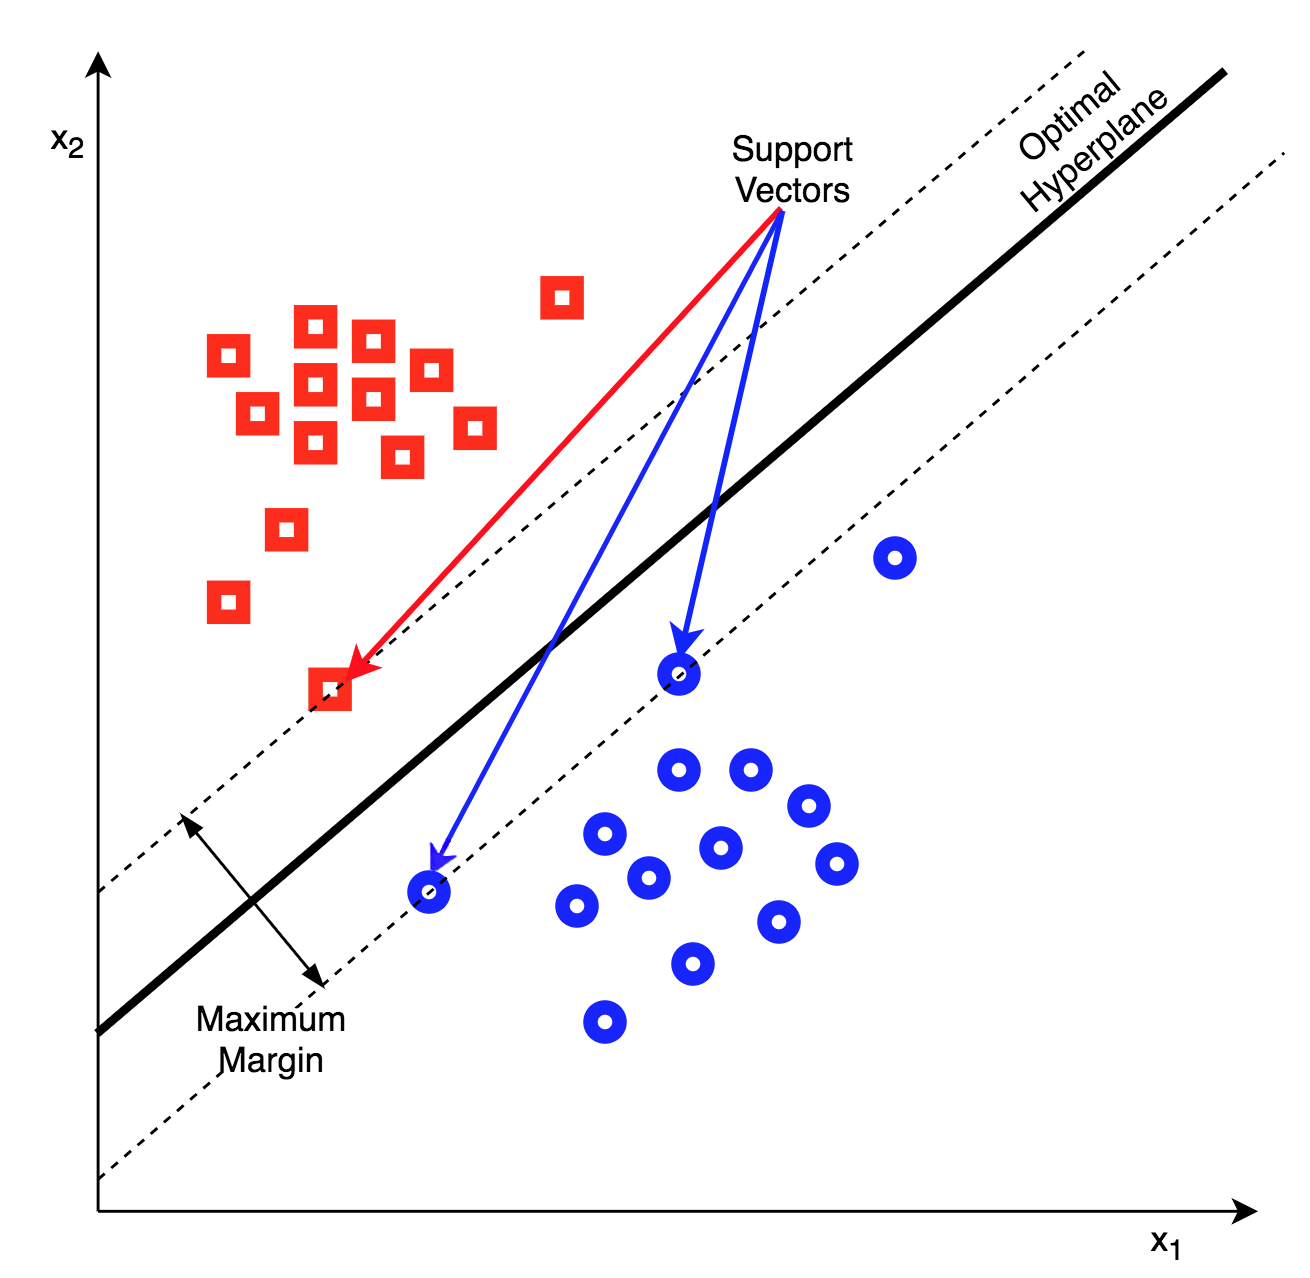
\includegraphics[width=0.7\linewidth]{Background/svm_vis.png}}
\caption{Visualization of the Optimal Hyperplane Learned by an SVM }
\label{svmvis}
\end{figure}

An SVM can use a kernel function to map the input data into higher dimensional space. Depending on the mapping, it is possible to further separate the distance between classes. This means that an SVM can learn nonlinear decision surfaces, given the right kernel. One of the most popular kernels to use is the radial basis kernel. The radial basis kernel projects the data onto a Taylor series expansion of a gaussian distribution.
